\begingroup\setstretch{1.22}
\section{Giao diện người dùng Desktop Cozy Harbor và Web Dash}

\subsection{Chọn màn và chơi thủ công}

Cozy Harbor hiển thị tọa độ, tên, nghề nghiệp, trạng thái đã chứng minh và lời khai trên thẻ đang mở. Từ menu hồ sơ, người chơi chọn một trong sáu màn hoặc mở tệp JSON. Chọn một thẻ úp để gửi phán quyết tội phạm hoặc vô tội. Khi chứng minh thành công, thẻ lật để lộ lời khai tiếp theo.

\begin{figure}[H]
\centering
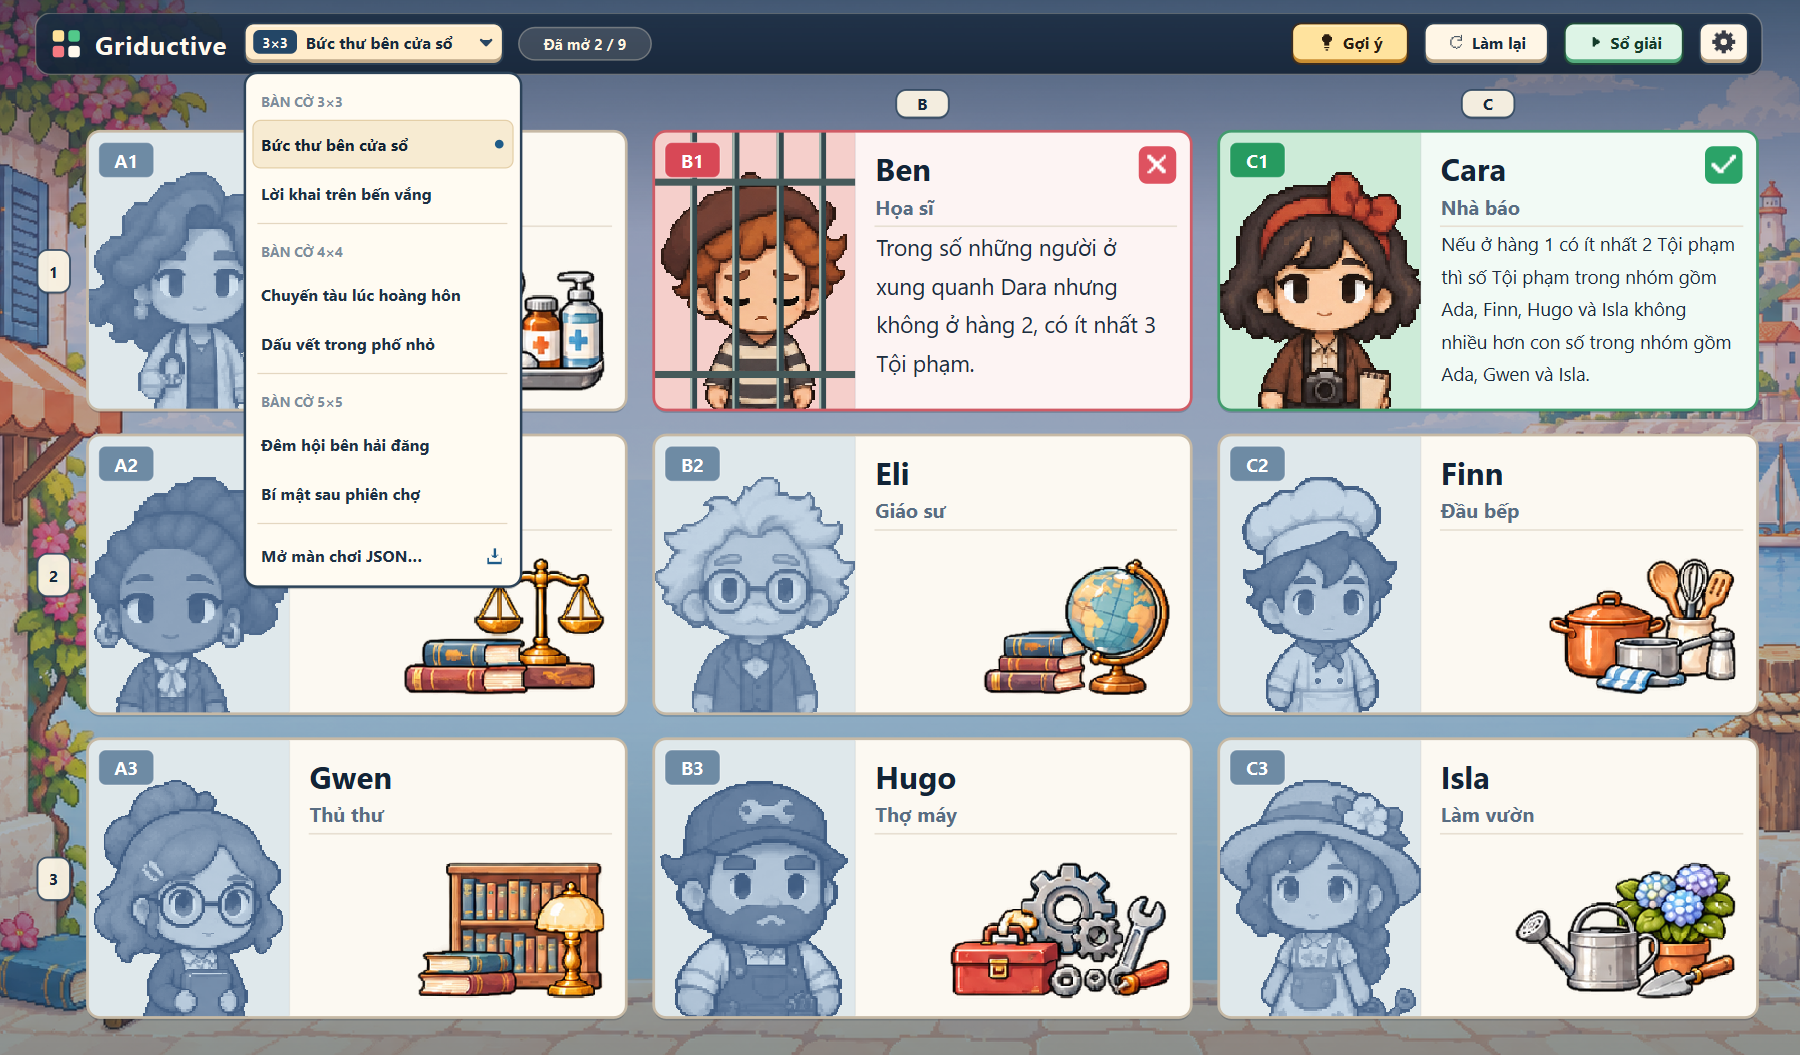
\includegraphics[width=0.78\linewidth]{img/ui_3x3_casemenu.png}
\caption{Menu hồ sơ trên bàn $3\times3$. Các màn được nhóm theo kích thước bàn.}
\end{figure}

Gợi ý xác định nhân vật có thể chứng minh tiếp theo từ cùng ảnh chụp công khai. Nút “Xem nhân vật” dẫn người chơi đến thẻ cần xét. Thao tác xem gợi ý giữ nguyên số thẻ đã mở.

\begin{figure}[H]
\centering
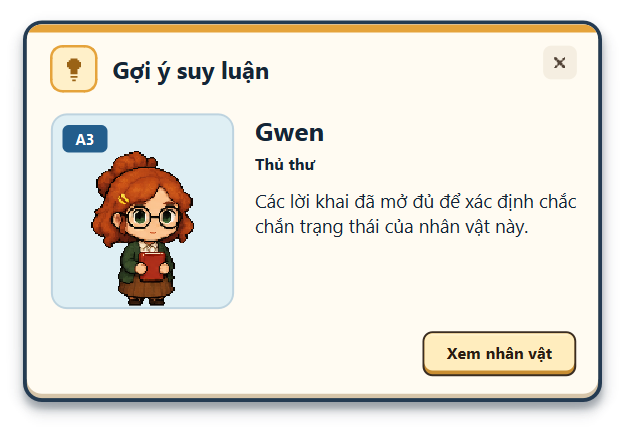
\includegraphics[width=0.34\linewidth]{img/ui_hint_modal.png}
\caption{Hộp gợi ý chỉ đến Gwen, thủ thư ở A3, khi các lời khai đã đủ để xác định trạng thái của cô.}
\end{figure}

\clearpage

\subsection{Đọc lời khai và theo dõi quá trình giải}

\begin{figure}[H]
\centering
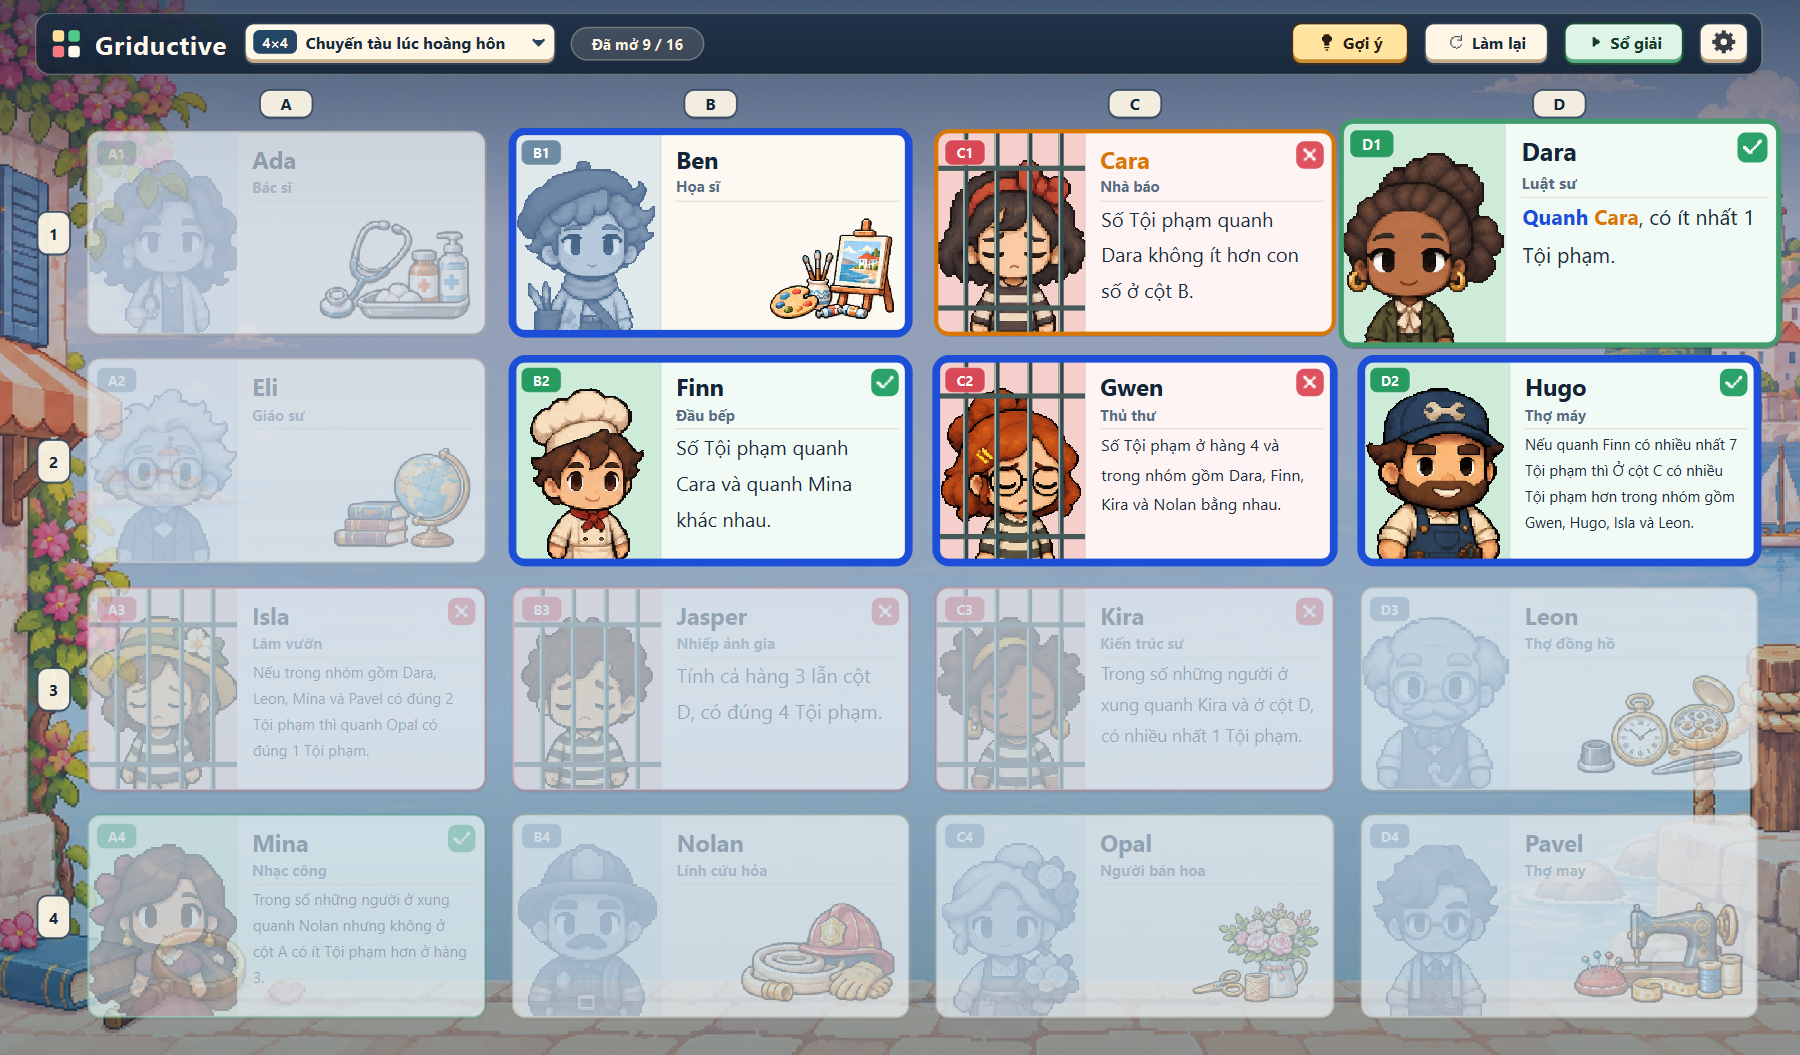
\includegraphics[width=0.75\linewidth]{img/ui_4x4_highlights.png}
\caption{Bàn $4\times4$ khi chọn lời khai. Viền màu xác định các ô thuộc vùng tham chiếu, còn các ô ngoài vùng được làm mờ.}
\end{figure}

Với lời khai nhiều vùng, màu của từng cụm từ khớp với đường viền trên bàn. Chọn hoặc ghim một vùng giúp đọc đúng toán hạng của phép so sánh. “Tự giải” lần lượt thực hiện các bước đã chứng minh. “Làm lại” khởi tạo lại màn từ những thẻ mở ban đầu.

\begin{figure}[H]
\centering
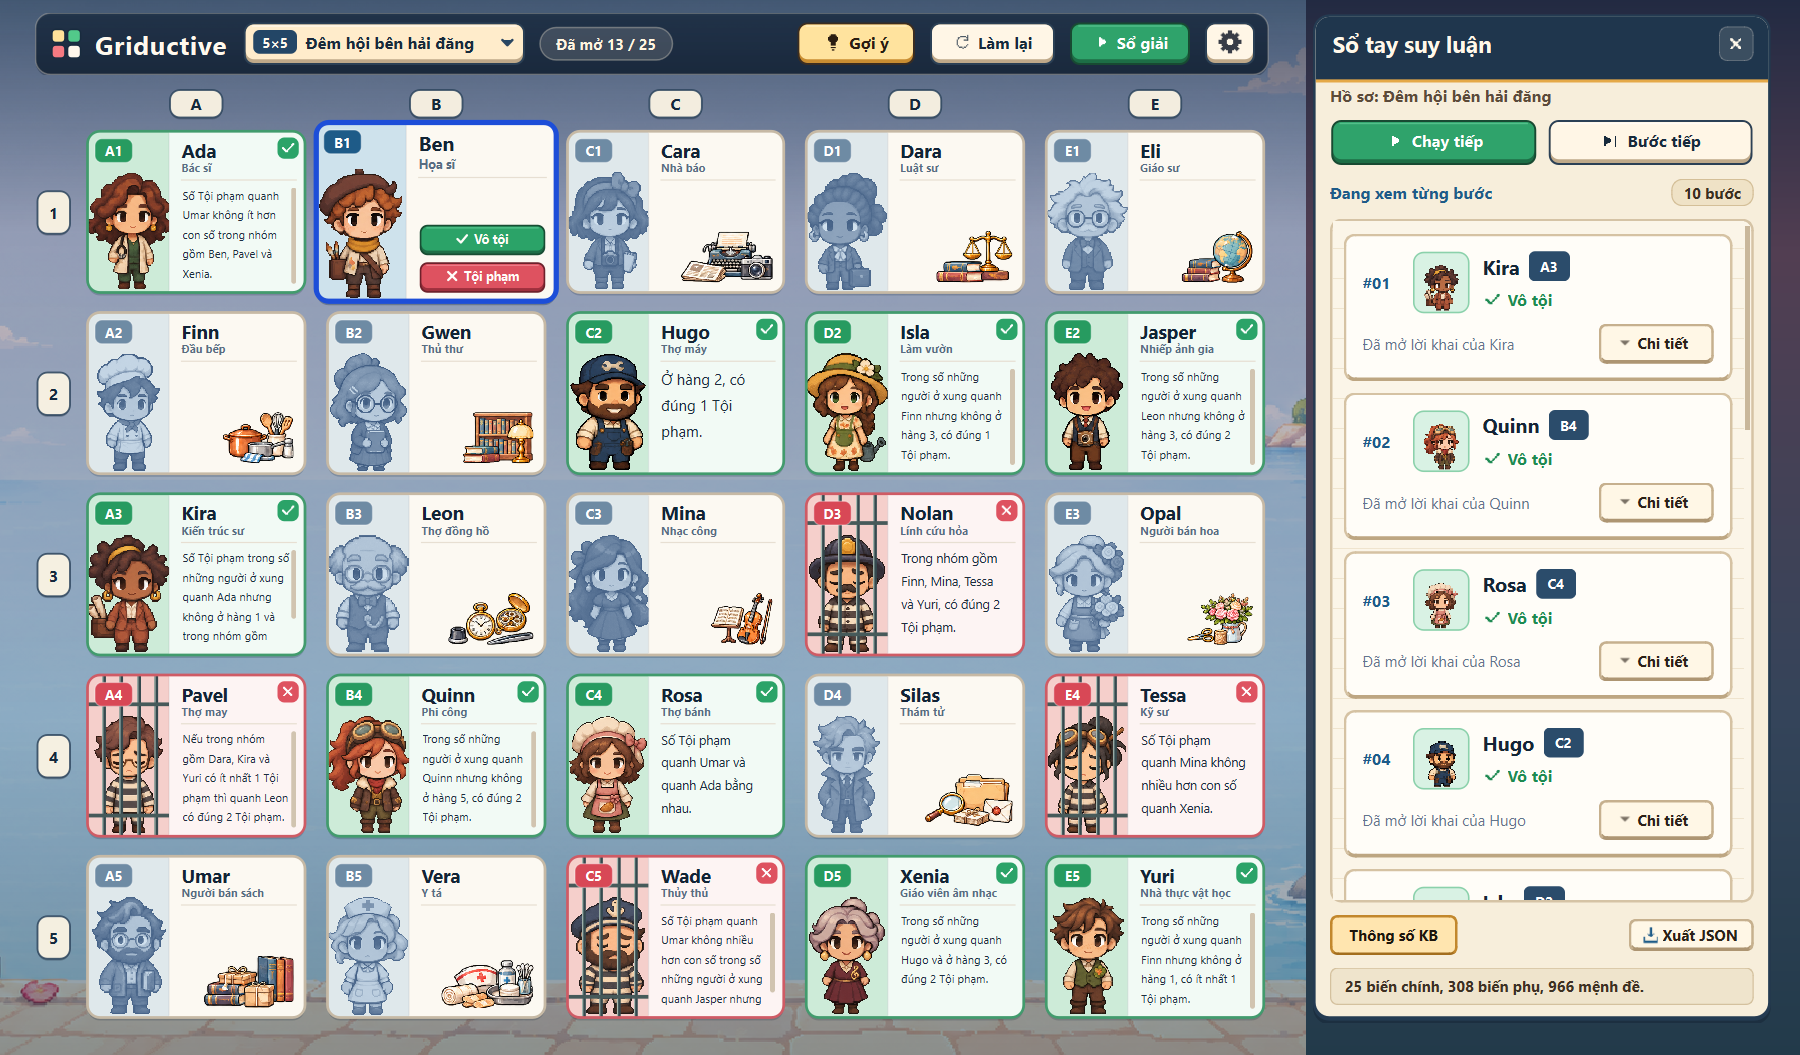
\includegraphics[width=0.75\linewidth]{img/ui_5x5_solver.png}
\caption{Bàn $5\times5$ bên cạnh sổ tay suy luận. Mỗi mục ghi ô vừa được xác định và có nút xem chi tiết.}
\end{figure}

\clearpage

\subsection{Phiên chơi Web Dash}

Giao diện Web dùng callback của Plotly Dash \cite{dashdocs} để nhận thao tác, dựng lại bàn và trả phần hiển thị công khai. Với màn có sẵn, \texttt{dcc.Store} ở chế độ \texttt{session} lưu mã màn, lịch sử nước đi và lựa chọn hiển thị. Đáp án và manh mối chưa mở nằm ở máy chủ. Nếu người chơi tự nạp tệp JSON, dữ liệu phiên còn giữ bản tệp do chính họ cung cấp để tái dựng màn.

Mỗi callback tạo một GameEngine cho phiên, kiểm tra kiểu dữ liệu và giới hạn số nước trong lịch sử theo số ô. Máy chủ phát lại từng đề nghị qua \texttt{submit}. Một nước thiếu chứng minh hoặc bị sửa sẽ khiến lịch sử bị từ chối. Chỉ sau khi tái dựng thành công, callback mới xử lý thao tác mới. Các phiên có thể đọc cùng bộ câu đố bất biến nhưng không chia sẻ tiến độ chơi.

Ví dụ, tự thêm A3 vào lịch sử phía trình duyệt chỉ có hiệu lực nếu máy chủ chứng minh được phán quyết tại đúng thời điểm đó. Đoán đúng đáp án ẩn vẫn chưa đủ để mở lá bài. Bộ kiểm thử Web gửi yêu cầu callback thật, kiểm tra từ chối lịch sử giả và xác nhận dữ liệu trả về cho màn tích hợp sẵn không chứa nghiệm ẩn.

Tệp tùy chỉnh được kiểm tra mã hóa, giới hạn 128 000 byte sau giải mã và được đọc qua một tệp tạm trước khi đưa vào bộ nạp câu đố chung. Cả Desktop và Web đều dùng chung phép chứng minh và điều kiện chấp nhận. Desktop giữ phiên trên worker, còn Web trả chi phí phát lại lịch sử để có thể xử lý yêu cầu kế tiếp trong tiến trình mới.

\par\endgroup
